\chapter{Cel projektu}

Celem realizowanego projektu było:

\begin{itemize}
	\item Udostepnienie serwisu odszukiwania scieżek w grafach.
	\item Umożliwienie wyboru różnych algorytmów planowania.
	\item Udostępnienie statystyk do ewaluacji dostarczanych algorytmów.
\end{itemize}

Serwis miał otrzymywać zlecenia w postaci grafu oraz węzła początkowego i końcowego, a następnie zwracać ścieżkę pomiędzy tymi punktami oraz meta-informacje związane z procesem obliczania ścieżki.

\section{Motywacja projektu}

Stworzony system może zostać wykorzystany w kilku różnych scenariuszach użycia:
\begin{itemize}
	\item Ewaluacja działania różnych algorytmów dla wybranego typu grafów.
	\item Ewaluacja wybranego algorytmu planowania dla różnych rodzajów grafów.
	\item Określenie wymagań czasowych i pamięciowych dla konkretnych problemów planowania
\end{itemize}

\section{Poszukiwanie ścieżek}

Problem poszukiwania możliwie optymalnej ścieżki w grafie sprowadza się do wyznaczenia zbioru węzłów lub zbioru krawędzi (istotne dla multigrafów) poprzez które można dostać się z węzła początkowego do węzła końcowego.
Interesują nas zwykle ścieżki, dla których sumaryczna wartość wag mijanych krawędzi będzie najmniejsza.
Rysunek \ref{fig:planowanie} przedstawia działanie algorytmu planowania dla przykładowego garfu.

\begin{figure}[!h]
	\centering
	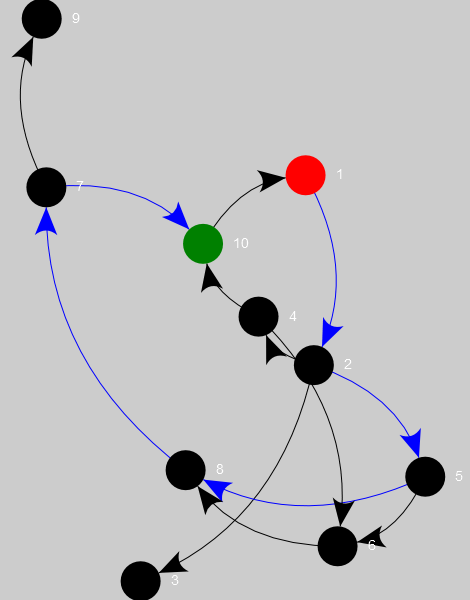
\includegraphics{img/planowanie.png}
	\caption{Przykład wyszukiwania ścieżki w grafie.}
	\label{fig:planowanie}
\end{figure}